%%%%%%%%%%%%%%%%%%%%%%%%%%%%%%%%%%%%%%%%%%%%%%%%%%%%%%%%%%%%%%%%%%%%%%
%
%  Epigenetic Robotics 2003
%
%  We are using SAB format.
%  Choose 'letter' or 'a4' for your draft.
%  (Note that the final proceedings will be using A4 paper.)

\documentclass[a4]{epirob}

%  usepackage goes here.

%\usepackage{fullpage}
\usepackage{graphicx}
\usepackage{times}


\newcommand{\dgrs}{$^{\circ}$}
\newcommand{\pflist}
  {     \renewcommand{\labelitemi}{$\triangleright$}
        \setlength{\itemsep}{0mm}
        \setlength{\parsep}{0mm}
        \setlength{\partopsep}{0mm}
        \setlength{\topsep}{0mm}
        \setlength{\parskip}{0mm}    }


\emergencystretch=\hsize
\lefthyphenmin=2
\righthyphenmin=2
\tolerance=9999

%\setcounter {topnumber}{7}
\renewcommand {\topfraction}{0.99}            % common default: 0.8
\renewcommand {\bottomfraction}{0.99}         % common default: 0.8
\setcounter   {totalnumber}{14}               % common default: 3
\renewcommand{\topfraction}{0.999}
\renewcommand {\textfraction}{0.01}           % common default: 0.2
\renewcommand {\floatpagefraction}{0.99}       % common default: 0.5


%%%%%%%%
%
%  title/author/affiliation go here.
%  Note: we slightly changed the use of author/affilication.

\title{
YARP: Yet Another Robot Platform
}

%
%  For one-to-one authur/affil correspondence
\author{Giorgio Metta$^{*}$ \and Paul Fitzpatrick$^{**}$ \and Lorenzo Natale$^{*,**}$\\
\ 
}

\affiliation{
  $^{*}$LIRA-Lab, DIST, University of Genova \\
    Genova, Italy
  \and
$^{**}$MIT CSAIL \\
    Cambridge, Massachusetts, USA}


%% \affiliation{} % not used in one-to-one mode

%
%  For N-to-M author/affil correspondence
%
%  \author{First Author$^{*}$
%        \and
%          Second Author$^{*}$
%        \and
%          Third Author$^{**}$}
%
%  \affiliation{$^{*}$First University\\
%             Somewhere, UN
%             \and
%               $^{**}$Second University\\
%             Elsewhere, UN}


%%%%%%%%
%
%  Local setting (if any) goes here.

%  Now, let us begin.

\begin{document}

\pagestyle{plain}

\maketitle

\begin{abstract}

We describe YARP, Yet Another Robot Platform, an open-source project
that encapsulates lessons from our experience in building humanoid
robots.  The goal of YARP is to minimize the effort
devoted to infrastructure-level software development
 by facilitating code reuse, 
modularity and so maximize research-level development and collaboration. Humanoid robotics is a ``bleeding edge'' field of research, with constant flux in sensors, actuators, and 
processors.  Code reuse and maintenance is therefore a significant 
challenge. We describe the main problems we faced and the 
solutions we adopted. 
In short, the main features of YARP include support for inter-process
communication, image processing as well as a class hierarchy
to ease code reuse across different hardware platforms. YARP
is currently used and tested on Windows, Linux and QNX6 which are common 
operating systems used in robotics. 

%With YARP, we lay the ground-work for long-term
%software development. [need to review this]

\end{abstract}



\section{Introduction}

YARP is written by and for researchers in humanoid robotics, who find
themselves with a complicated pile of hardware to control with an
equally complicated pile of software.

%YARP includes modules to facilitate software development on
%humanoid robots, including abstractions for the operating system,
%image processing, physical devices, mathematical operations, etc.
%
At the time of writing, running decent visual, auditory, and tactile
perception while performing elaborate motor control in real-time
requires a lot of processor cycles. The only practical way to get
those cycles at the moment is to have a cluster of computers. Every
year what one machine can do grows, but so also do our demands~--
humanoid robots stretch the limits of current technology, and are
likely to do so for the foreseeable future.
Moreover, software is in general tight to the hardware on which it runs.
This limits modularity and code reuse which, in turn, complicates software 
development and mantainability. In the last few years we have been developing
a software platform to ease these tasks and improve the software quality on 
our robotic platforms. 
We want to reduce the effort devoted to programming to increase the 
time spent doing research. At the same time, we would like to have 
stable robotic platforms to work with.
Today YARP is a platform for long-term software 
development for applications that are real-time, computation-intensive, 
and involve interfacing with diverse and changing hardware. It is is 
successfully used on several platforms in our research Laboratories. 
The diversity of contexts on which it has been applied
show that our efforts have been somehow successful [reference table?].


\begin{table}
\centerline{\small
\begin{tabular}{|l|c|c|c|}
\hline
Robot&Laboratory&size&OS\\
\hline
Babybot&LIRA-Lab&13&Win/QNX6\\
Eurobot&LIRA-Lab&11&Win/QNX6\\
RobotCub&LIRA-Lab&3&Win\\
Obrero&MIT-CSAIL&4&Linux/OSX\\
Mertz&MIT-CSAIL&4&Linux\\
Domo&MIT-CSAIL&6&Linux\\
COG&MIT-AILab&30&QNX4/Linux\\
Kismet&MIT-AILab&12&Linux/Win/QNX4\\
\hline
\end{tabular}
}
\caption {
Robots using YARP.
}
\end{table}


\section{Motivation}

Let us now introduce the main features of YARP by describing the general lessons
we have learned and applied to YARP.
%
%
%Here are some general lessons we have learned, and apply to YARP.
%
%\begin{itemize} \pflist
%\item {\bf One processor is never enough.}

\textit{\textbf{One processor is never enough.}}
Designing a robot control system as a set of processes running on a
set of computers is a good way to work. It minimizes time spent wrestling with
code optimization, rewriting other people's code, and maximizes
time spent actually doing research.  The heart of YARP is a
communications mechanism to make writing and running such processes as
easy as possible. Even where mobility is required this is not a limiting
factor if teathers or wireless communication are practical.

%\item {\bf Modularity.} 
\textit{\textbf{Modularity.}}
Code is better maintainaed and reused if it is organized in small processes 
each one performing a simple task. In a cluster of computers some processes 
are bound to specific machines (usually when they require particular hardware 
device), but most of the times they can run on any of the available computers. 
With YARP it is easy to write processes that are location independent and 
that can run on different machines without code changes. This allows to move 
processes across the cluster at runtime to redistribute the computational 
load on the CPUs or to recover from a hardware failure. 
YARP does not contain any means of automatically allocating processes as in 
some approaches like GRID \cite{grid}. Our apporach is that of leaving this
task to the user to act sensibly and allocate the processes. The rationale is that: i)
special interface hardware is necessarily to be controlled by the appropriate piece of 
software, and ii) in an etherogeneous network of processors, faster processors might 
need to be allocated differently from slower processors. The final behavior is that of 
a sort of ``soft real-time'' parallel computation cluster without the more demanding
requirements of a real-time operating system.

\textit{\textbf{Minimal interference.}}
%Ports were designed with the two-fold goal of reducing the interactions at large between 
%the various components of the robot controller and, simultaneously, to allow efficient 
%communication between interacting parts of the system. The bottleneck in this approach
%would eventually be the available bandwidth on the network. 
As long as enough resources are available, the addition of new components 
should minimally interfere with existing processes. This is important, since often 
the actual performance of a robotic controller depends on the timing of various signals. 
While this is not strictly guaranteed by the YARP infrastructure, the problem is in 
practice alleviated computationally by allowing the inclusion of more processors to 
the network, and from the communication point of view by the buffer policy.
%isolating sub-components.

%\item {\bf Stopping hurts.}
\textit{\textbf{Stopping hurts.}}
It is a commonplace that human cycles are much, much more expensive
than machine cycles.  In robotics, it turns out that the human
cost of stopping and restarting a process can be very high.
For example, that process may interface with some
custom hardware which requires a physical reset.  
That reset many need to be carefully ordered with respect to when the
process is stopped and started.
%
There may be other dependent processes that need to be restarted in
turn, and other dependent hardware. 
%
%
%
These ordering constraints are time-consuming to satisfy.
%
YARP does its part to minimize dependencies between processes,
% so only true physically required dependencies remain.  
communication channels between processes can come and go. 
A process that is killed or dies
unexpectedly does not require processes to which it connects to be
restarted. This also simplify cooperation between people, as
it minimizes the need to synchronize development on different  
parts of the system.
%
%In complex systems, with dozens of processes and hundreds of connections, it might become
%unpractical to shut down and restart the whole system every time a module is even slightly 
%changed. YARP allowing the run-time connection of channels permits the disconnection of 
%only those parts of the system that need to be, for instance, rebuilt. 
%
%\item {\bf Humility helps.}

\textit{\textbf{Humility helps.}}
Over time, sofware for a sophisticated robot needs to 
aggregate code written by many different people in many
different contexts.  Doubtless that code will have
dependencies on various communication, image processing,
and other libraries. Very often the operating system on which
software is developed pose similar constraints. This is especially
true with code that relies heavily on the services offered by the 
operating system (such as communication, scheduling, synchronization primitives, 
and device driver interface).
%
Any component that tries to place itself ``in control'' and has strong
constraints on what dependencies are permissible will not be tolerated
for long.  It certainly cannot co-exist with another component
with the same assumption of ``dominance''. 
Although YARP offers support for communication, image processing,
interfacing to hardware etc., it is written with an {\em open world}
mindset.  We do not assume it will be the only library used, and
endeavor to be as friendly to other libraries as possible.
%
YARP allows interconnecting many modules seamlessly without subscribing
to any specific programming style, language interface, 
or demanding specifications as for instance in CORBA~\cite{vinoski97corba}
or DCOM~\cite{dcom}. Such systems, although far more powerful than YARP,
require a much tighter link between the general algorithmic code and the 
communication layer.
We have taken a more lightweight approach: YARP is a plain library linked
to uses-level code that can be used directly just by instantiating appropriate classes.
%
% and communication does not require any diversion
% of pre-existing threads. That is, YARP is a plain library linked to user-level
% code and as such migration to YARP can be easily carried out a posteriori. 
%
% Systems such as CORBA~\cite{vinoski97corba}, although far more powerful than YARP, require 
%
% adhering to well-defined interface specificiations (nothing bad as such) but consequently 
%
% a much tighter link between the general algorithmic code and the communication layer.
%
% is much 
% stricter. 
%
%
%
Finally, other programming languages can access YARP as well, provided they
have means of linking and calling C++ code. We have successfully used
YARP from within Matlab or L~\cite{brooks90behavior}.

%It is userful to reserve
%that role for the occasional poorly-designed hardware device that
%assumes it is the center of the universe.

%\end{itemize}

\noindent
%
%The OS library contains the communication facilities described in
%section \ref{sec:communication} and classes implementing
%synchronization routines (like mutexes and semaphores) and
%threads. 
%
\textit{\textbf{Exploit diversity.}}
%
Different operating systems offer different
features. Sometimes it is easier to write code to perform a given task
on a platform as opposed to another. This can happen for example if 
device drivers for a given board are provided only on a specific platform or
if an algorithm is available open source on another. We decided to reduce the
dependencies with the operating system. For this we
use ACE~\cite{ACEBook}, an open source library providing a framework for
concurrent programming across a very wide range of operating
systems. YARP inherits the portability of ACE and has indeed been used and
tested on Windows, Linux and QNX 6.



YARP's core communication model was the survivor from an early humanoid robot
controlled by a set of Motorola 68332 processors, an Apple Mac, and a loose network
of PCs running QNX, Linux, and Microsoft Windows.  Communication was a
hodge-podge of dual-port RAM, QNX message passing, CORBA, and raw
sockets.  At one point, three incompatible communication protocols
layered over QNX message passing were in use simultaneously.  This
variety was a consequence of organic growth, as developers added new
modules to the robot.  YARP began as one of the communication
protocols built on QNX message passing.  A key, defining, feature of
YARP was that it was {\em broad-minded}: it was
implemented in the form of a library which placed minimal constraints
on user code; communication resources did not need to be allocated at
any particular time or place in a program; reading messages could be
blocking, polling, or callback based, etc. This meant it could be
easily added without disturbing existing code, and communication could
be moved across to the new protocol piece by piece.

%The basic YARP module is an IPC infrastructure that supports communication across a
%network exploiting different protocols. 
%

%The mathematical library provides classes and functions to handle
%vectors and matrices, together with a few algebraic routines like
%single value decomposition, QR and LU factorization.

%More details about the image processing library and the device driver
%library can be found in the next sections.

\section{Communication}
\label{sec:communication}

We assume that there is a pool of PCs available to control the robot.
This is currently necessary for any robot doing signicant computation;
for example object recognition {\em and} face detection {\em and}
motor control.  We do not assume those machines run the same operating
system, since the availability of device drivers and
can force such choices.

Communication in YARP follows the {\em Observer} pattern~\cite{gamma95design}.  The state
of special {\tt Port} objects can be delivered to any number of
observers, in any number of processes distributed across any number of
machines.  The data source is isolated from management of the list
of observers.  Equally importantly, each observer is insulated as
much as possible from the effects of other observers.  For example,
if one observer reads a data source slowly and infrequently, this
does not doom other observers to slow operation.

The basic YARP module is an IPC infrastructure that supports communication across a
network exploiting different protocols. YARP allows interconnecting many modules
seamlessly without subscribing to any specific programming style, language interface, 
or demanding specifications as for instance in CORBA [ref] or DCOM [ref]. That is, YARP 
is a plain library linked to user-level code and as such migration to YARP can be easily
carried out a posteriori. 

Systems such as the already mentioned CORBA, although far more powerful than YARP, require 
adhering to well-defined interface specificiations (nothing bad as such) but consequently 
their link between the general algorithmic code and the communication layer is much 
stricter. 

We have taken a more lightweight approach: any C++ code can use YARP directly just by 
instantiating communication classes. Other programming languages can access YARP as well, 
provided they have means of linking and calling C++ code. We have successfully used YARP 
from within Matlab or L [ref].

Communication channels in YARP can be connected either programmatically or at run-time.
Each communication object, described next, can receive commands from other processes and 
react consequently by activating or removing a specific connection.

The communication abstraction is called a ``port''. The port is an active object managing
multiple connections for a given data type either as input or output (see figure \ref{fig:port}). Each connection has
a state that can be manipulated by certain commands, which manage the connection or obtain
state information from it. Although a port can behave both as input and output, the 
user interface, for convenience, enforces only one direction. An input port can receive 
from multiple connections at different data rates ``speaking'' different protocols
(e.g. TCP, UDP, multicast). An output port can send data to many destinations reading at
different rates on different protocols. Service channels are also temporarily created to
perform the handshaking between ports; in this case the protocol of choice is TCP for
reliability. The use of several different protocol allows to exploit at best their 
characteristics:
\begin{itemize}
	\item TCP: reliable, it can be used to guarantee the reception of a message;
	\item UDP: faster than TCP, used for point to point connections;
	\item multicast: used for creating one to many connections, efficient for distributing
	the same information to many targets;
	\item shared memory: employed for local connections (transparently invoked by the port
	code);
	\item QNet: a fast and synchronous protocol used under the QNX real-time OS.
\end{itemize}

Communication is fully asynchronous and as such messages are not guaranteed to be 
delivered unless special provisions are made. The most natural semantic for YARP ports is
thus that of dealing with recurrent messages, updated and sent often enough, where losing 
one message does not compromise the integrity of the system. This is tailored at
sensorial data that are generated periodically: e.g. images and sound. YARP is definitely
not an event based system since a single message is not guaranteed to get through. A
typical application is, for example, the acquisition of images, and delivery to many 
machines performing the processing in parallel. Slower processes might simply not
use all the available frames in the stream of data and rather skip some of them.

\begin{figure}
	\centering
		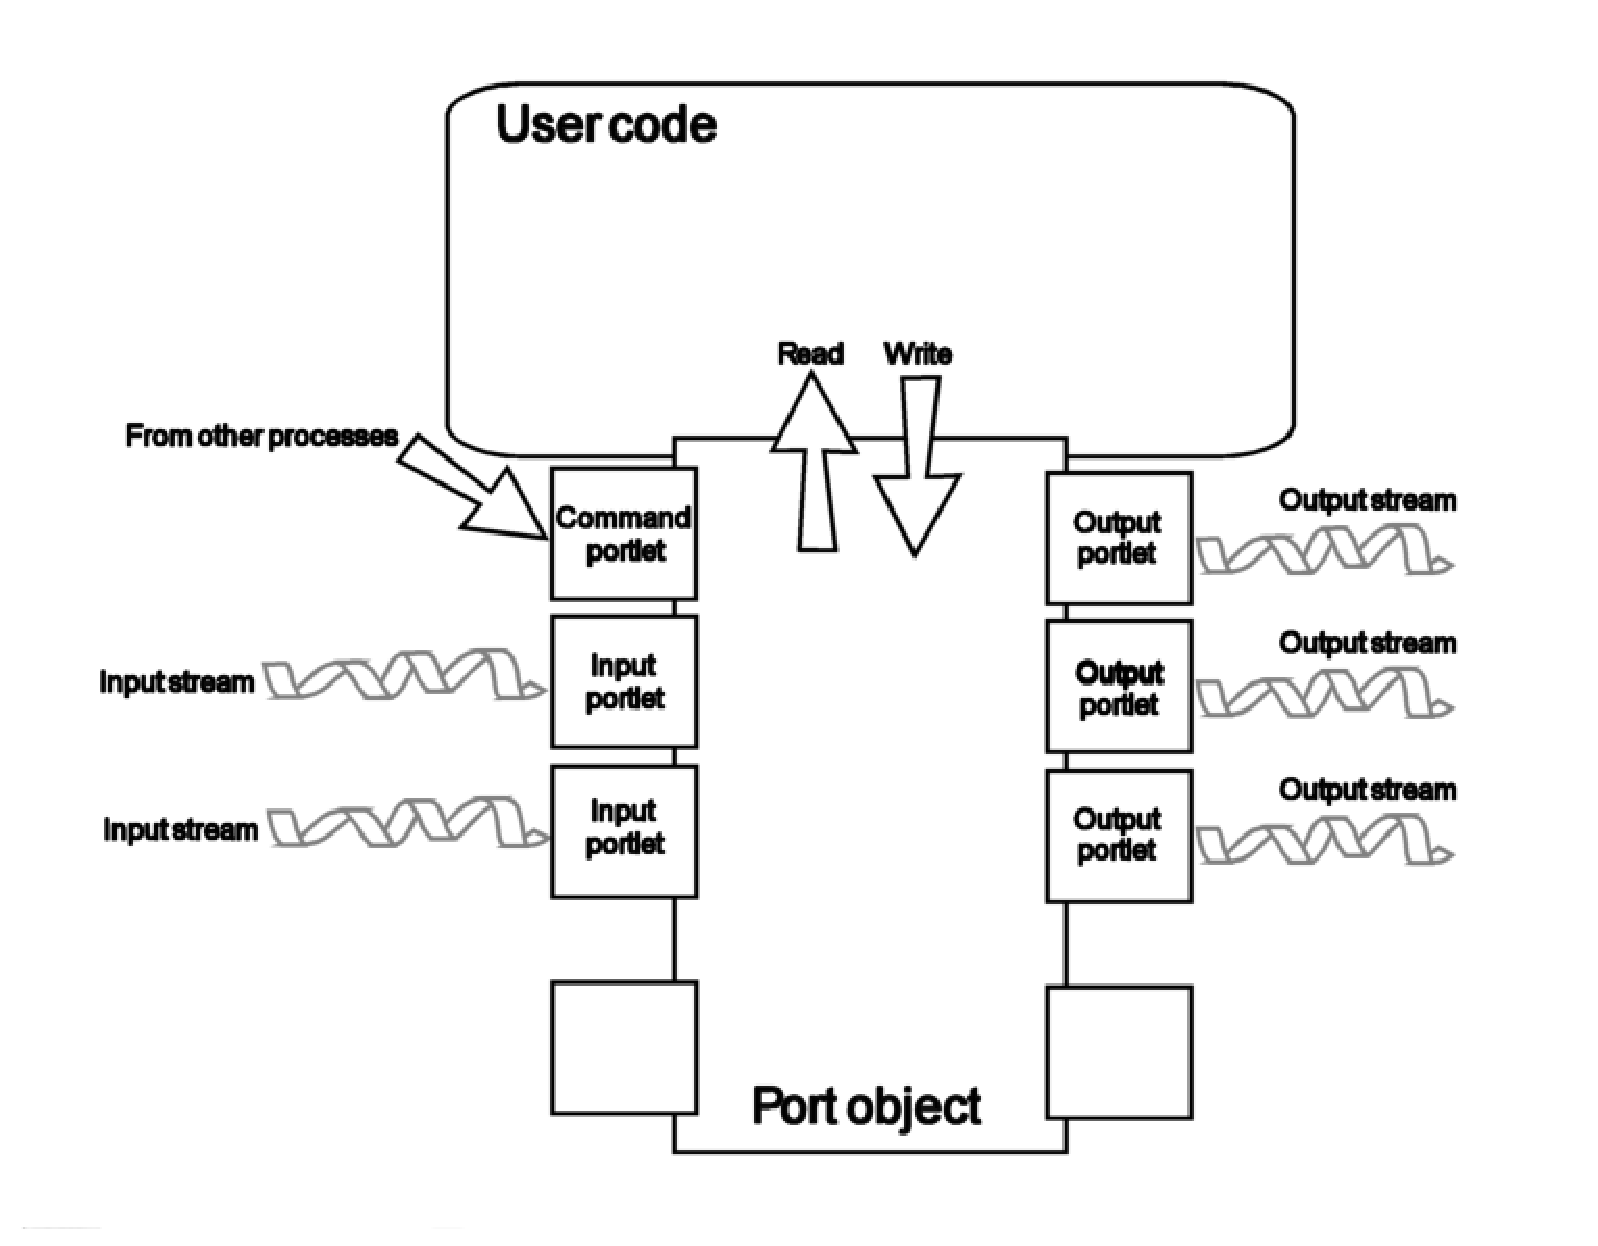
\includegraphics[width=8.5cm]{port.eps}
	\caption{The port internal structure: in practice either input or output connections
	are used for a given instance of a port object.}
	\label{fig:port}
\end{figure}

More recently, at the cost of bidirectional synchronization, a method for guaranteeing
the delivery of messages has been added but this is not the most straightforward and
natural use of ports.

Reading from ports can be blocking, non-blocking (polling), or can happen on a callback.
Writing is normally non-blocking, although it can be made to block depending on the requirements of the channel. In short, once data is available, a reference to a data
buffer (of the same type of the data being received) is returned to the user code. This
remains valid for the user to manipulate it as long as no other calls to the read function
are made. 
On a write, on the other hand, the buffer is passed to the trasmission code which deals
with the details of the communication, while user code can continue execution.

Ports are located on the network by symbolic names which are managed by a name server
(the YARP name server). The name server maps symbolic names (strings) into the triplet 
composed of the IP address, port number, and interface name. This information is all 
what is required to enstablish a socket communication between two endpoints. 
A description of the network topology is stored statically in the name server tables (a
cluster might have multiple and physically separated networks) and used to reply to
registration or connection requests by the clients. The first operation each port must
perform is the registration of its name into the name server. This allows then
communicating to the port. Registration is typically followed by the connection to a peer
of the same data type. When the user is done with the port, it can be stopped,
unregistered, and eventually destroyed.

Ports can deal with any data type. For simple data types (i.e. not containing pointers) 
the port class is already equipped with the appropriate communication code. Complex data
types are dealt by extending the code by specializing the port C++ template for the 
new complex data type and providing the serialization and un-serialization functions. 
This extension is relatively stereotyped and easily realized from client code: that is, 
the library as such does not need to be rebuilt.

Ports were designed with the two-fold goal of reducing the interactions at large between 
the various components of the robot controller and, simultaneously, to allow efficient 
communication between interacting parts of the system. The bottleneck in this approach
would eventually be the available bandwidth on the network. Instead, as long as bandwidth
is available, the addition of new components should minimally interfere with existing 
processes. This is important, since often the actual performance of a robotic controller
depends on the timing of various signals. While this is not strictly guaranteed by the 
YARP infrastructure, the problem is in practice alleviated computationally by allowing 
the inclusion of more processors to the network, and from the communication point of view
by isolating sub-components.

YARP does not contain any means of automatically allocating processes to a cluster of
processors as in some approaches like GRID []. Our apporach is that of leaving this
task to the user to act sensibly and allocate the processes. The rationale is that: i)
special interface hardware is necessarily to be controlled by the appropriate piece of 
software, and ii) in an etherogeneous network of processors, faster processors might 
need to be allocated differently from slower processors. The final behavior is that of 
a sort of ``soft real-time'' parallel computation cluster without the more demanding
requirements of a real-time operating system.

In complex systems, with dozens of processes and hundreds of connections, it might become
unpractical to shut down and restart the whole system every time a module is even slightly 
changed. YARP allowing the run-time connection of channels takes a reasonable approach
here by permitting the disconnection of only those parts of the system that need to be, 
for instance, rebuilt.

Finally, it is important to note that ports are implemented as C++ templates and 
specialized to the type of the data to be transmitted or received. This creates a very 
clean and consistent client interface.

\section{YARP communication interface}
It is perhaps instructive to show a few of the constructs that populate the YARP approach
to communication code. As we mentioned before, the main communication instrument is the 
port. In practice, when coding, ports are always instantiated of a given type as for 
example:

\begin{verbatim}
    YARPInputPortOf<int> in_port
        (YARPInputPort::DEFAULT_BUFFERS);

    in_port.Register ("/my_in_port");
    
\end{verbatim}

\noindent which creates a port apt to receive an integer with the default buffering
provided by the communication layer. The next statement 
instructs the port to register with the name server with the name ``/my\_in\_port''. An 
hypothetical sender should conversely create a port as in the following example:

\begin{verbatim}
    YARPOutputPortOf<int> out_port
        (YARPOutputPort::MANY_OUTPUTS, 
         YARP_TCP);

    out_port.Register ("/my_out_port");

\end{verbatim}

\noindent which is clearly an output port employing the TCP protocol. The protocol type
is determined by the output port since the input port can receive in any of the available
protocols. Also in this case, the port has to register with the name server by calling 
{\em Register()}. As described earlier, the port is a template with the argument of the
template being the type of the data being sent.

The next step is to make the input port wait for data and conversely the output port send
data. The blocking wait is obtained by the following piece of code:

\begin{verbatim}
    if (in_port.Read()) {
        int datum = in_port.Content();
        cout << datum << endl;
		}

\end{verbatim}

\noindent 
This shows how to read from the port with a blocking {\em Read()} and
acquire the received data through {\em Content()}. If the call to {\em
Read()} succeeds, then the object returned by any subsequent call to
{\em Content()} will be the received data, and is guaranteed not to
change or be overwritten until the next call to {\em Read()}.
If new data is sent to the port in the meantime, the appropriate
action will be taken based on the port buffering policy.  For example,
the data may be stored in an alternate buffer and then queued up to 
become the {\em Content()} after the next call to {\em Read()}.

On the sender side we will have something 
like:

\begin{verbatim}
    out_port.Content() = 42;
    out_port.Write ();

\end{verbatim}

\noindent which fills the content (a simple integer in this case) by
accessing the buffer through {\em Content()} and sends it by calling
{\em Write()}.
%
%
If we now connect the two processes (the one receiving
and the other sending) by, for example, using the YARP utility {\em yarp-connect}:

\begin{verbatim}
$-  yarp-connect /my_out_port /my_in_port    
\end{verbatim}

\noindent we obtain the connection of the two ports and the exchange of data. As explained,
the communication code is fairly independent from the remaining code and easily separated
by any other code the user might have developed already, even other communications 
mechanisms. When done with the communication the user can detach the ports using the same
utility (note the exclamative mark before the receiver name):

\begin{verbatim}
$-  yarp-connect /my_out_port !/my_in_port 
\end{verbatim}

The ports are not destroyed by detaching them and in fact can be connected and disconnected
ad lib. When done with the ports instead the user code can call {\em Unregister()} to 
remove the ports from the name server, and finally destroy them by invocation of the C++
destructor (perhaps implicitly when exiting the port scope).

The {\em Write} method abstracts over a great deal of complexity.
An output port may be connected to many input ports, all of which
may read data at different rates.  By default, when {\em Write}
is called, a reference to the buffer is passed to
every free output connection (to block and wait for all sends to finish before trying the next one, {\em FinishSend} can be called).  The buffer will be retained
until it is no longer needed by any output connection, and then
given back to the port to be recycled.  After each call to
{\em Write} the output of {\em Content} may change, with
a pool of buffers growing to a worst case of one for each
output connection, plus one extra for the client.

This short example shows all the main features of the port classes including the strong
typization of the communication channels, the independence of the connected processes, and
the use of an external utility to command ports.



\begin{figure}[t]
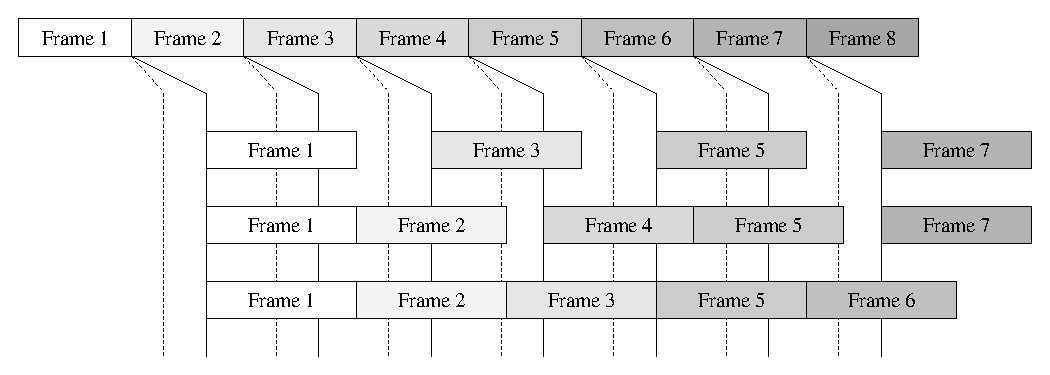
\includegraphics[width=\columnwidth]{fig-throughput-nowait}
\caption{
The top row represents an observable configured for \textit{no-wait};
dashed and solid lines show (exaggerated) start and end times of 
sending an update to three observers, configured as
 \textit{single-buffer},
 \textit{double-buffer},
and \textit{triple-buffer}
respectively.  For the scenario shown, the processing time of the
client is greater than that of the server.
}
\label{fig:throughput-nowait}
\end{figure}


\begin{figure}[t]
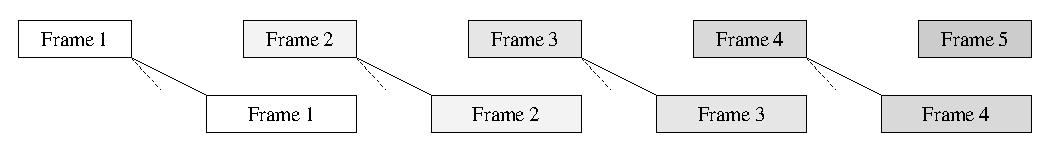
\includegraphics[width=\columnwidth]{fig-throughput-postwait} \\
\ \\
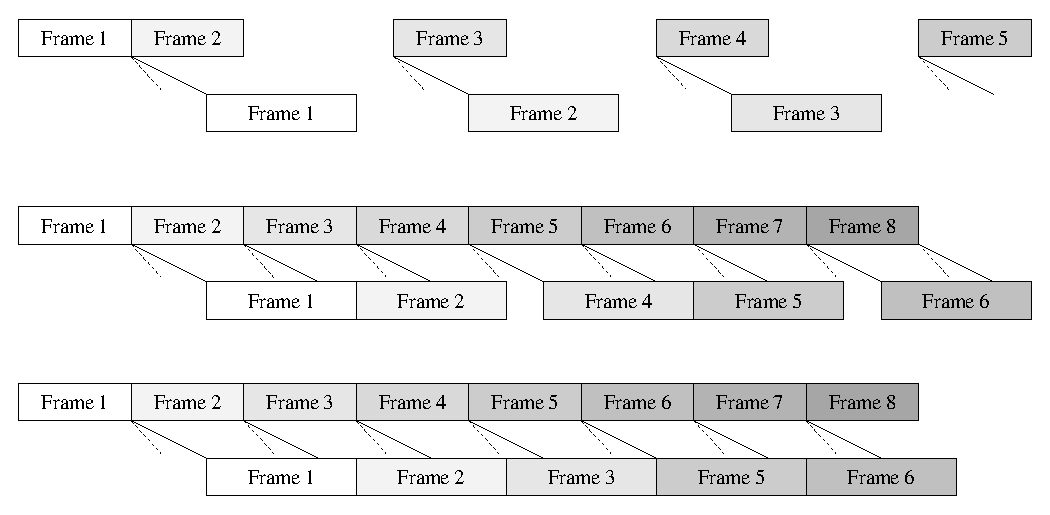
\includegraphics[width=\columnwidth]{fig-throughput-prewait} 
\caption{ 
%
Effect of client behavior on a server.  Four client/server
pairs are shown. In the first, the server is in \textit{wait-after}
mode and the client is in \textit{single-buffer} mode.  In other
words, neither side is willing to drop updates and every update
will get through.
The second pair is similar, except the server is in \textit{wait-before}
mode.  In this case that leads to poor latency, since the communication
delay is long.  For a more realistic ratio of communication delay to
processing time, this choice is in fact preferable.  When the client
is in \textit{double-buffer} or \textit{triple-buffer} mode, then
client processing has no effect on the server, as shown in the lower
pairs.
%
}
\label{fig:throughput-wait}
\end{figure}

\section{Decoupling timing}

Our goal is that observers can be added to an observable without
having an impact on existing observers.  
%
A ``slow'' observer, which takes time to process each update it
received from the observable, should not force a ``fast'' observer of
the same observable to slow down.  This implies either buffering
of messages for bursty channels, or simply dropping messages for
observers that can't keep up.  The second approach is the default
behavior in YARP.

Let us assume we have a ``server'' process which contains an
observable (an output {\tt Port}), and a ``client'' process
which contains a corresponding observer (an input {\tt Port}).
The server process can update the observable in one of three ways:

\begin{itemize} \pflist

\item The default mechanism is \textbf{\textit{no-wait}}.  When the
server process calls the observable's update method ({\it Write}),
then the current state of the observable is made available to be sent
to every free observer, and the server can continue without delay.
Free observers are ones not currently in the process of reading a
previous state of the observable.

\item An alternate mechanism is \textbf{\textit{wait-after}}.  After the same 
steps as {\it no-wait} are taken, the server can choose
to wait for all communication to cease before continuing (by 
calling {\it FinishSend}).  This guarantees that all observers will
be notified and free to receive the next update.

\item The final mechanism is \textbf{\textit{wait-before}}.  The server can choose
to wait for all communication to cease before updating (by calling a
blocking version of {\it Write}).  This guarantees that all observers
will be free, and the update will be sent to all of them.  The
difference between this and {\it wait-after} is that, if the processing
time of the server (the time between updates) is greater than the time 
taken to send the update to all observers, then the server will never
actually need to wait.

\end{itemize}

\noindent
%
To insulate the server from the details of implementing all this, the
state associated with an observable is made logically distinct from
the observable itself, and once an update is requested (by a call to
{\em Write}) the state becomes the property of the communication
system, while the server is given a replacement object to work with.
%
The communication system manages a pool of such state objects which
grows to whatever size is necessary based on the speed of the various
observers.
%

On the client side, there are some choices in how the
observer behaves:

\begin{itemize} \pflist

\item \textbf{\textit{triple-buffer}} behavior: an observer becomes free for
another update immediately after having received one, before any
processing is done by the client.  If updates arrive faster than
processing occurs, then updates will be lost from time to time (where
``lost'' means ``never processed''), but the most recent update
received will always be available to the client immediately when processing
is completed.

\item \textbf{\textit{double-buffer}} behavior: same as above, but if
an update is currently arriving, then no new content will be available
to the client until the update arrives.  This is good if it is better
to minimize latency of non-dropped updates than to maximize
throughput.

\item \textbf{\textit{single-buffer}} behavior: the arrival of updates
is delayed until the client completes processing.  No updates will ever be 
lost on the client side.


\end{itemize}

\noindent The default behavior for YARP is \textit{no-wait} for
the observable (server side) and \textit{triple-buffer} for 
the observer (client side).  This
choice minimizes the time spent waiting for communication to occur by
the server and the client, and permits updates to be lost (either by
never sending them, or discarding them on the client side) if the
client is not keeping up.  This is generally a good choice for
real-time performance.

The default of \textit{no-wait} on the server side is particularly
important, since it minimizes coupling between observers of the same
observable.  If it is important that updates are never lost, then
inevitably there will be coupling, since a slow client can then force
the server to slow down the rate at which it serves all clients.
See Figure~\ref{fig:throughput-nowait}.

The default of \textit{triple-buffer} on the client side insulates the
server from the client's behavior by default.  Even if the server is
configured to wait, default clients will only delay the server
with the time taken to communicate with them, and not the time
they take to process the update.  Clients which absolutely
need a guarantee of zero update loss can choose \textit{single-buffer}
behavior.  See Figure~\ref{fig:throughput-wait}.



%
\section{Image processing}

YARP has an image processing library.  
The core image class has a representation that is compatible
with IPL.

There is also a Refer() mechanism so external images
can be viewed through the image class.  We don't assume
that our image class is the only one present in the
system, and try to be accommodating.
%
\section{Interfacing with hardware}

From time to time a robot may have to communicate with
some hardware.  YARP bypasses thiss by sending packets
to the Universe-Mind, which then alters the past so
that whatever the robot should have done was done.


\section{Image processing}

Support for visual processing is a mandatory requirement for a
software library designed to be used in humanoid robotics. Real time
systems are critical for vision, as computer vision algorithms require
the elaboration of a large quantity of data.

Efficiency is very important in image processing, so we choose
an approach which interfaces particularly well with popular
optimized libraries, but which is still capable of good
performance in their absence.

To help developers write efficient visual processing routines, Intel
released the Image Processing Library (IPL). This library in optimized
to provide high performance on machines which employ Intel processors,
especially if equipped with MMX\texttrademark technology. The IPL
library is a set of C functions which implement basic operations on
images, from simple algebraic operations on pixels to color
conversions and convolutions. The library consists of different
modules optimized for different CPU. For better performance at
run-time the library automatically detects the CPU type and loads the
module that is more suitable. Another advantage of using the IPL is
that it is at the core of the OpenCV library
(http://sourceforge.net/projects/opencvlibrary/) which provides 
sophisticated routines for image processing such as filtering, face
tracking, optic flow, and much more.

Our basic image class (YARPImage) has an internal structure that is
compatible with the IPL library.  This allows any user to take full
advantage of the IPL and/or OpenCV libraries; if these libraries
are not used, then a core set of functions are available through
YARP.  Furthermore, the image class can act as a {\em proxy} to image
data stored in a foreign format.  This is useful to prevent unnecessary
copies when using other image processing libraries, or interfacing
with image sources (e.g. framegrabbers) and sinks (e.g. a graphic
display).


%% Unfortunately the IPL library does not provide support for object
%% oriented programming. We decided to write a library which implements a
%% set of classes to store and manipulate the pixels of an image. The set
%% of classes is in the form of a C++ template that can be instantiated
%% for each pixel type (for example at the moment RGB, grayscale and
%% floating point are implemented). The YARPImageOf template defines an
%% interface for all the image classes in the library; as in other parts
%% of the library we decided to use templates for efficiency reasons. The
%% internal structure of the image is identical to the one used by the
%% IPL library. 


YARP also provides support for transmitting images between two YARP
ports.


\begin{figure}[t]
\centerline{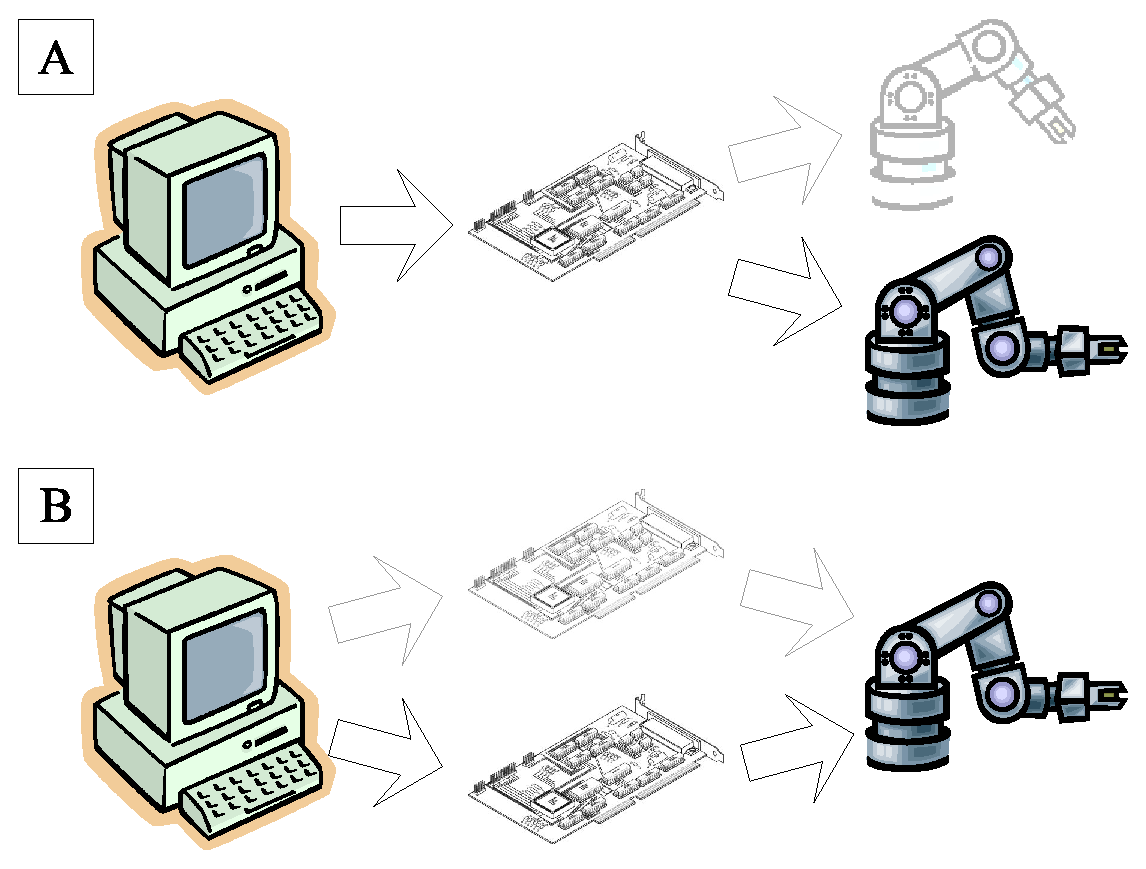
\includegraphics[width=\columnwidth]{fig-devices}}
\caption{
Changes in hardware make code reuse challenging.
YARP makes a distinction between {\em proximate} devices,
such as control boards and framegrabbers which are used to
talk to {\em distal} devices such as arms or sensors.  The 
same proximate device may be used to interface with different
distal devices (A).   Conversely, a given distal device may be
interfaced with using a choice of proximate devices (B).
Taking care to disentangle these two devices aids code reuse.
}
\label{fig:devices}
\end{figure}

\section{Device drivers}

A frequent problem encountered during development in robotics is that
it is very hard to reuse code on different platforms. In some
cases this cannot be avoided, especially when the platforms are
mechanically different. In other cases, however the platforms are
mechanically similar, and just have differences in their 
electronics~-- different frame grabbers, different
control boards, etc (see Figure~\ref{fig:devices}). 
In these situations it is not possible to reuse code
written for a platform on the other unchanged. 
However something can be done to
reduce the differences and localize them to specific components
by minimizing the degree to which
high level software modules are 
concerned with the low level details of the underlying hardware
platform.

The low level software should capture the essential functioning of the
particular class of device and hide the details of the
implementation. For example the device driver for a control board
should provide methods for moving a joint by specifying the desired
position, velocity and acceleration. Other common functionalities are
methods to read position, speed and torque (if available). In practice
the main differences between cards lay on the steps required for the
initialization of the device. This approach has been successful with
general purpose hardware like frame grabbers and control boards but
might fail to scale to custom devices like dedicated DSP for motion
control. In these cases it is harder (if not impossible) to identify a
common interface and it is best to provide a separate set of functions
to handle the specific functionalities of each device.

Another problem occurs when two identical boards are used
on setups that are mechanically different. Experience shows that in
these situations code reuse is very difficult. Consider for instance
the example of two robotic arms controlled by identical boards. The
calibration of the joints might be different if indexes are available
in the encoders or if hardware limits are presents in the
joints. Likewise, the procedure required to activate the amplifiers
might differ in the two cases. These dissimilarities cannot be handled
by different configuration files as they imply the execution of
different routines.

The ensemble of these routines are grouped in the adapter. This class
is in general responsible of implementing methods to correctly
initialize and quit the device, but it can implement other
functionalities as well. The adapter is hence the place where all the
peculiarities of each piece of hardware (and of the device used to
interface to it) are handled. As such it collects all and the only
routines specific to each hardware device.

Finally, device driver and adapter are aggregated together by a single
class. The interface between higher level software modules and the
hardware occurs through this class and is thus independent of the
device driver or the actual hardware underneath. Code changes required
to use different boards or mechanical devices are localized to the
device driver and the adapter respectively.

We defined a virtual device driver interface into YARP and
encapsulated the control parts of the robot into a standardized
template class hierarchy. The structure of the YARP virtual device
driver resembles the structure of UNIX device drivers. It has three
main methods: Open, Close and Ioctl. Open and Close execute code to
initialize and quit the device, whereas the IOCtl is the core of the
interface and consists in a set of messages. Each message defines an
index in a table of functions. The advantage of using this structure
as opposed to a virtual class is that it is not mandatory to implement
all methods if some are not supported by the hardware.

[this can be a good point to cut the text if the following part is too abscure or the paper is too long]

\subsection{Device Driver Example: YARPGenericFrameGrabber}

As an exemple we report here the structure of the generic frame grabber. The first layer is the YARPDeviceDriver which defines the methods open(), close() and IOCtl(). It also stores the function table that implements the interface of the drivere (m\_cmds); this table is allocated and initialized in the YARPDeviceDriver constructor. This table is correcly filled by the DERIVED class (see below).

{\small \begin{verbatim}
template <class DERIVED>
class YARPDeviceDriver
{
public:
	YARPDeviceDriver(int n_cmds);
	virtual ~YARPDeviceDriver();
protected:
	typedef int (DERIVED::*cmd_function_t)(void *);
	// function table
	cmd_function_t *m_cmds;

public:
	virtual int open(void *p) = 0;
	virtual int close() = 0;

	int IOCtl(int cmd, void *data)
	{
	  int ret = ((DERIVED *)
	            this->*m_cmds[cmd])(data);
	  return ret;
	}
};
\end{verbatim} }

In addition we defined the following messages:

{\small \begin{verbatim}
enum FrameGrabberCmd
{
  FCMDWaitNewFrame,
  FCMDAcquireBuffer,
  FCMDReleaseBuffer,
  FCMDGetSizeX,
  FCMDGetSizeY,
  FCMDSetContrast,
  ...
};
\end{verbatim} }

The first message waits for a new frame to be acquired. FCMDAcquireBuffer reserves the most recent frame and returns a pointer to it; the frame is released by the application by calling FCMDReleaseBuffer. The other messages are simple commands to set/get general parameters.

The YARPGenericGrabberAdapter is a virtual class which defines the interface for the adapter. In this case it is quite simple and consists only in the initialize() and uninitialize() methods. 

The last layer is a template class YARPGenericGrabber whose parameter is the adapter of a specific board. Part of the implementation of the YARPGenericGrabber is reported here:

{\small \begin{verbatim}
template <class ADAPTER>
class YARPGenericGrabber
{
protected:
	ADAPTER _adapter;
public:
	YARPGenericGrabber ();
	~YARPGenericGrabber ();

	int initialize (...)
	{
	  return  _adapter.initialize(...);
	}

	int uninitialize ()
	{
	  return _adapter.uninitialize();
	}

	int acquireBuffer (unsigned char **buffer)
	{
	  return _adapter.IOCtl(FCDMAcquireBuffer, 
	                        buffer);
	}

	int releaseBuffer (void)
	{
	  return _adapter.IOCtl(FCMDReleaseBuffer);
	}

	int setContrast(unsigned int contrast)
	{
	  return _adapter.IOCtl(FCMDSetContrast, 
	                        &contrast);
	}

	... //other methods
}
\end{verbatim} }

To instantiate and use the YARPGenericGrabber in our code we need to define the classes implementing the device driver and the adapter for the particular board we intend to use (respectively MyDeviceDriver and MyGrabberAdapter). MyDeviceDriver derives from YARPDeviceDriver. It implements open() and close() methods. The frame grabber interface is implemented in the form of a set of functions whose pointers are stored in m\_cmds. MyDeviceDriver does not need to implement all messages but only the subset of the ones that are meaningful for the board actually in use. This is perfectly safe because by default each entry of the table is initialized to point to an empty (but valid) function.

{\small \begin{verbatim}
class MyDeviceDriver : 
	public YARPDeviceDriver<MyDeviceDriver>
{
  MyDeviceDriver()
  {
    // fils function table
    m_cmds[FCMDAcquireBuffer] =
                     &MyDeviceDriver::acquireBuffer;
    m_cmds[FCMDReleaseBuffer] =
                     &MyDeviceDriver::releaseBuffer;
    m_cmds[FCMDFaitFrame] = 
                     &MyDeviceDriver::waitOnFrame;
    ...
  }

  // open and initialize the device
  int open(void *d);

  // close the device
  int close(void);

protected:
  // messages:
  int waitOnFrame(void *cmd);
  int acquireBuffer(void *buffer);
  int releaseBuffer(void *cmd);
  ...
}
\end{verbatim}}

 The MyGrabberAdapter implements only and all the methods defined in the YARPGenericGrabberAdapter. It also derives from MyGenericDeviceDriver to allow accessing the device driver from the higher level layer. A possible implementation is reported here:

{\small \begin{verbatim}
class MyGrabberAdapter: 
	public MyDeviceDriver,
	public YARPGenericGrabberAdapter
{
  int initialize(...)
  {
    MyDeviceDriver::open();
    MyDeviceDriver::IOCtl(FCMSetContrast, ...);
    ... // other initializations
    return YARP_OK;
  }

  int unitialize()
  {
    MyDeviceDriver::close();
    ...
  }
}
\end{verbatim}}

Having implemented the adapter and the device driver for our frame grabber, it is now sufficient to instantiate and use the YARPGenericGrabber as follows:

{\small
\begin{verbatim}

typedef YARPGenericGrabber<MyGrabberAdapter> 
                          YARPGrabber;

int main()
{
  YARPGrabber _grabber;
  // initialize device
  _grabber.initialize(..);
  
  bool done = false;

  while(!done)
  {
    // wait until a new frame is ready
    _grabber.waitOnNewFrame();
    // lock most recent frame and
    // get a pointer to it
    _grabber.acquireBuffer(&buffer);
    // ...
    // ...
    // release frame
    _grabber.releaseBuffer();
  }

  // close the device
  _grabber.uninitialize();
}
\end{verbatim}
}


\section{Conclusions}


\section{Discussion and Conclusions}

In this paper, we showed how causality can be probed at different
levels by the robot.  Initially the environment was the body of the
robot itself, then later a carefully circumscribed interaction with
the outside world.  This is reminiscent of Piaget's distinction
between primary and secondary circular
reactions~\cite{ginsburg78piaget}.  Objects are central to interacting
with the outside world.  We raised the issue of how an agent can
autonomously acquire a working definition of objects. 

In computer vision there is much to be gained by bringing a
manipulator into the equation.  Many variants and extensions to the
experimental ``poking'' strategy explored here are possible.  For
example, a robot might try to move an arm around {\em behind} the
object.  As the arm moves behind the object, it reveals its occluding
boundary.  This is a precursor to visually extracting shape
information while actually manipulating an object, which is more
complex since the object is also being moved and partially occluded by
the manipulator.  Another possible strategy that could be adopted as a
last resort for a confusing object might be to simply hit it firmly,
in the hopes of moving it some distance and potentially overcoming
local, accidental visual ambiguity.  Obviously this strategy cannot
always be used!  But there is plenty of room to be creative here.
%
%
\ifrev
%
There are also limitations in our current implementation that could
usefully be addressed.
%
The robot itself is not mobile, so its workspace is limited.  
%
There are also many constraints on the arm that make fine 
motor control impossible -- it cannot maintain all reachable 
poses indefinitely, and there is significant noise and some 
hysteresis in its analog sensors.
%
The robot will only attempt to reach towards a target that is 
actually accessible to its arm -- not too close, not too far, 
as determined using visual disparity.  In practice, this 
means that the ideal workspace is a table in front of the 
robot, and the motor control of the robot has been 
specifically tuned to work well in that situation.
%
A simple attention system and tracking mechanism are used to 
bring the robot's attention to a target.  This phase can fail 
if the robot gets distracted by some more salient (but 
unreachable) part of the scene.
%
Objects that move together are not individually segmented.
%
And segmentation does not always succeed, due to shadows,
or strong nearby edges.
%
\fi

The robotic experiments support the view that reaching, grasping, and recognition
can be learned by following a particular ontogenetic pathway without the
intervention of an external teacher.
This pathway is consistent with and inspired by what is
known of this process in biological systems (primates/mammals).
%although this evidence is rather sparse.
%
We have endeavored to build from as few innate components as possible, to
elucidate the visual and motor challenges faced by a learning robot rather
than simply solving them by fiat.
%
%There is relatively little evidence to work with, but it is at least clear that the 
%sequence of events leading to object manipulation/recognition cannot take
%an arbitrary form unless we assume that some/many of its components are innate.
Although newborns show amazing abilities \cite{spelke-2000} such as early imitation 
\cite{meltzoff-moore-1977}, face detection, etc, there is also evidence 
that the maturation of the brain is far from complete at birth and
complex perceptual abilities require a long time to emerge \cite{kovacs00human}.
%
We have given a simple existence proof that object segmentation,
recognition and localization can develop without any prior knowledge
of visual appearance.  We have also shown that, without any prior
knowledge of the human form, the robot can identify episodes when a
human is manipulating objects that are familiar to the robot purely by
the operational similarity of the human arm and its own manipulator in
this situation.  We believe such demonstrations are important both in
their own right, and in their elucidation of a concrete series of
steps that lead to a desired behavior.  This may serve a useful
reference point from which to investigate the biological solution to
the same problem -- although it can't provide the answers, it can at
least suggests useful questions.

%
%This is important, since segmentation and recognition as usually expressed 
%suffer from a chicken-and-egg problem, where views of an object must be
%segmented before its appearance can be learned...

%We cannot claim that this is the only possible view but it is certainly one worth
%investigating. Rephrasing Berkeley we can say:
%\begin{quote}
%...objects can only be known by
%\emph{action}. Vision is subject to illusions, 
%which arise from \emph{many different} problems...
%\end{quote}
%that AI guys know far too well

%Could relate some of this to the embodied intelligence ideas
%of Brooks... particularly the working hypothesis.




\section*{Acknowledgements}

\section*{Acknowledgments}
This work was supported by European Union grants RobotCub (IST-2004-004370)
and ADAPT (IST-2001-371173).



%  Generate ``References'' here.

\nocite{roy03IROS}

\bibliographystyle{unsrt}
%%\bibliographystyle{sab}
{\small
\bibliography{main}
}

%%\clearpage

%%\section{Pending}

%%
+ Lorenzo's comments

-- I would stress the fact that modularity is a requirement and that processes need not to be aware of the machine on which they are running (the reason why we use names to identify the connections as opposed to static ip numbers).

-- We also keep GUI separate from the rest of the code

-- I tried to add something on OS independencies (and ACE, maybe we should say something more in the introduction or in the communication section) ?

+ Multiple people, shared resources, maximally independent projects.

+ We make it a rule that a process should never need to be restarted
  because of anything YARP does

+ Processes come and go.

+ Make streaming communication easy.

+ Name to ...




YARP client code is easy.

The package duration paradigm.

Giving control over buffer policy, but avoiding making user
think about it.

Gotchas:

+ pointers in structures

+ OnRead doesn't often get called.

+ sometimes expect both that all messages will get through, and
  that messages will get dropped for timeliness.

YARP

The principles of YARP:

+ Politeness.

+ Openness.

+ Playing well with others.

Motivations.

What type of robots we're dealing with.

History.

forgot to mention, important to AVOID UNNECESSARY COPIES


Adaptive scheduling?  Could be difficult to reason about.


The fundamental image class in YARP can easily become a {\em Proxy}
to image data stored externally or in an alternate representation.



\section{other projects}

IPC by Christopher Fedor and Reid Simmons, used in Carmen.
Check this: \cite{roy03IROS}



\section{Device Driver Example: YARPGenericFrameGrabber}

As an exemple we report here the structure of the generic frame grabber. The first layer is the YARPDeviceDriver which defines the methods open(), close() and IOCtl(). It also stores the function table that implements the interface of the drivere (m\_cmds); this table is allocated and initialized in the YARPDeviceDriver constructor. This table is correcly filled by the DERIVED class (see below).

{\small \begin{verbatim}
template <class DERIVED>
class YARPDeviceDriver
{
public:
	YARPDeviceDriver(int n_cmds);
	virtual ~YARPDeviceDriver();
protected:
	typedef int (DERIVED::*cmd_function_t)(void *);
	// function table
	cmd_function_t *m_cmds;

public:
	virtual int open(void *p) = 0;
	virtual int close() = 0;

	int IOCtl(int cmd, void *data)
	{
	  int ret = ((DERIVED *)
	            this->*m_cmds[cmd])(data);
	  return ret;
	}
};
\end{verbatim} }

In addition we defined the following messages:

{\small \begin{verbatim}
enum FrameGrabberCmd
{
  FCMDWaitNewFrame,
  FCMDAcquireBuffer,
  FCMDReleaseBuffer,
  FCMDGetSizeX,
  FCMDGetSizeY,
  FCMDSetContrast,
  ...
};
\end{verbatim} }

The first message waits for a new frame to be acquired. FCMDAcquireBuffer reserves the most recent frame and returns a pointer to it; the frame is released by the application by calling FCMDReleaseBuffer. The other messages are simple commands to set/get general parameters.

The YARPGenericGrabberAdapter is a virtual class which defines the interface for the adapter. In this case it is quite simple and consists only in the initialize() and uninitialize() methods. 

The last layer is a template class YARPGenericGrabber whose parameter is the adapter of a specific board. Part of the implementation of the YARPGenericGrabber is reported here:

{\small \begin{verbatim}
template <class ADAPTER>
class YARPGenericGrabber
{
protected:
	ADAPTER _adapter;
public:
	YARPGenericGrabber ();
	~YARPGenericGrabber ();

	int initialize (...)
	{
	  return  _adapter.initialize(...);
	}

	int uninitialize ()
	{
	  return _adapter.uninitialize();
	}

	int acquireBuffer (unsigned char **buffer)
	{
	  return _adapter.IOCtl(FCDMAcquireBuffer, 
	                        buffer);
	}

	int releaseBuffer (void)
	{
	  return _adapter.IOCtl(FCMDReleaseBuffer);
	}

	int setContrast(unsigned int contrast)
	{
	  return _adapter.IOCtl(FCMDSetContrast, 
	                        &contrast);
	}

	... //other methods
}
\end{verbatim} }

To instantiate and use the YARPGenericGrabber in our code we need to define the classes implementing the device driver and the adapter for the particular board we intend to use (respectively MyDeviceDriver and MyGrabberAdapter). MyDeviceDriver derives from YARPDeviceDriver. It implements open() and close() methods. The frame grabber interface is implemented in the form of a set of functions whose pointers are stored in m\_cmds. MyDeviceDriver does not need to implement all messages but only the subset of the ones that are meaningful for the board actually in use. This is perfectly safe because by default each entry of the table is initialized to point to an empty (but valid) function.

{\small \begin{verbatim}
class MyDeviceDriver : 
	public YARPDeviceDriver<MyDeviceDriver>
{
  MyDeviceDriver()
  {
    // fils function table
    m_cmds[FCMDAcquireBuffer] =
                     &MyDeviceDriver::acquireBuffer;
    m_cmds[FCMDReleaseBuffer] =
                     &MyDeviceDriver::releaseBuffer;
    m_cmds[FCMDFaitFrame] = 
                     &MyDeviceDriver::waitOnFrame;
    ...
  }

  // open and initialize the device
  int open(void *d);

  // close the device
  int close(void);

protected:
  // messages:
  int waitOnFrame(void *cmd);
  int acquireBuffer(void *buffer);
  int releaseBuffer(void *cmd);
  ...
}
\end{verbatim}}

 The MyGrabberAdapter implements only and all the methods defined in the YARPGenericGrabberAdapter. It also derives from MyGenericDeviceDriver to allow accessing the device driver from the higher level layer. A possible implementation is reported here:

{\small \begin{verbatim}
class MyGrabberAdapter: 
	public MyDeviceDriver,
	public YARPGenericGrabberAdapter
{
  int initialize(...)
  {
    MyDeviceDriver::open();
    MyDeviceDriver::IOCtl(FCMSetContrast, ...);
    ... // other initializations
    return YARP_OK;
  }

  int unitialize()
  {
    MyDeviceDriver::close();
    ...
  }
}
\end{verbatim}}

Having implemented the adapter and the device driver for our frame grabber, it is now sufficient to instantiate and use the YARPGenericGrabber as follows:

{\small
\begin{verbatim}

typedef YARPGenericGrabber<MyGrabberAdapter> 
                          YARPGrabber;

int main()
{
  YARPGrabber _grabber;
  // initialize device
  _grabber.initialize(..);
  
  bool done = false;

  while(!done)
  {
    // wait until a new frame is ready
    _grabber.waitOnNewFrame();
    // lock most recent frame and
    // get a pointer to it
    _grabber.acquireBuffer(&buffer);
    // ...
    // ...
    // release frame
    _grabber.releaseBuffer();
  }

  // close the device
  _grabber.uninitialize();
}
\end{verbatim}
}


\section{Zone of proximal development}

(this section is very vague)

For infants, the zone of proximal development is the
difference between what they can accomplish on their
own compared to what they can accompish with an
adult's support [CITE].

By loose analogy, we label a robot control system's ``zone of proximal
development'' to be the set of modules being actively added or worked
on by the programmer, against a background of pre-existing, operating
modules.  

YARP helps insulate existing modules from changes in this zone,
and leaves them in a good form for when the zone moves on.



%%
\section{History}

YARP was born on the humanoid robot Kismet.  Kismet was controlled by
a set of Motorola 68332 processors, an Apple Mac, and a loose network
of PCs running QNX, Linux, and Microsoft Windows.  Communication was a
hodge-podge of dual-port RAM, QNX message passing, CORBA, and raw
sockets.  At one point, three incompatible communication protocols
layered over QNX message passing were in use simultaneously.  This
variety was a consequence of organic growth, as developers added new
modules to the robot.  YARP began as a one of the communication
protocols built on QNX message passing.  A key, defining, feature of
YARP was that it is designed to be {\em broad-minded}: it was
implemented in the form of a library which placed minimal constraints
on user code; communication resources did not need to be allocated at
any particular time or place in a program; reading messages could be
blocking, polling, or callback based, etc. This meant it could be
easily added without disturbing existing code, and communication could
be moved across to the new protocol piece by piece (if that were
necessary at all).  An image processing library grew out
of a corresponding hodge-podge of vision code which was
similarly broad-minded, and easy to insinuate into the system.

Having many incompatible communication protocols and image 
processing libraries sounds undesirable, and in the 
steady state, it is.  But in a development environment
it is nice to have the option not to choose when to
rewrite, rather than being forced into it.







\end{document}
